\documentclass{ximera}
%\usepackage{todonotes}

\newcommand{\todo}{}

\usepackage{tkz-euclide}
\tikzset{>=stealth} %% cool arrow head
\tikzset{shorten <>/.style={ shorten >=#1, shorten <=#1 } } %% allows shorter vectors

\usepackage{tkz-tab}  %% sign charts
\usetikzlibrary{decorations.pathreplacing} 

\usetikzlibrary{backgrounds} %% for boxes around graphs
\usetikzlibrary{shapes,positioning}  %% Clouds and stars
\usetikzlibrary{matrix} %% for matrix
\usepgfplotslibrary{polar} %% for polar plots
\usetkzobj{all}
\usepackage[makeroom]{cancel} %% for strike outs
%\usepackage{mathtools} %% for pretty underbrace % Breaks Ximera
\usepackage{multicol}

\usepackage{polynom}



\usepackage[many]{tcolorbox}  %% for titled boxes
\newtcolorbox{xbox}[1]{%
    tikznode boxed title,
    enhanced,
    arc=0mm,
    interior style={white},
    attach boxed title to top center= {yshift=-\tcboxedtitleheight/2},
    fonttitle=\bfseries,
    colbacktitle=white,coltitle=black,
    boxed title style={size=normal,colframe=white,boxrule=0pt},
    title={#1}}


\usepackage{array}
\setlength{\extrarowheight}{+.1cm}   
\newdimen\digitwidth
\settowidth\digitwidth{9}
\def\divrule#1#2{
\noalign{\moveright#1\digitwidth
\vbox{\hrule width#2\digitwidth}}}





\newcommand{\RR}{\mathbb R}
\newcommand{\R}{\mathbb R}
\newcommand{\N}{\mathbb N}
\newcommand{\Z}{\mathbb Z}

%\renewcommand{\d}{\,d\!}
\renewcommand{\d}{\mathop{}\!d}
\newcommand{\dd}[2][]{\frac{\d #1}{\d #2}}
\newcommand{\pp}[2][]{\frac{\partial #1}{\partial #2}}
\renewcommand{\l}{\ell}
\newcommand{\ddx}{\frac{d}{\d x}}
\newcommand{\ddt}{\frac{d}{\d t}}

\newcommand{\zeroOverZero}{\ensuremath{\boldsymbol{\tfrac{0}{0}}}}
\newcommand{\inftyOverInfty}{\ensuremath{\boldsymbol{\tfrac{\infty}{\infty}}}}
\newcommand{\zeroOverInfty}{\ensuremath{\boldsymbol{\tfrac{0}{\infty}}}}
\newcommand{\zeroTimesInfty}{\ensuremath{\small\boldsymbol{0\cdot \infty}}}
\newcommand{\inftyMinusInfty}{\ensuremath{\small\boldsymbol{\infty - \infty}}}
\newcommand{\oneToInfty}{\ensuremath{\boldsymbol{1^\infty}}}
\newcommand{\zeroToZero}{\ensuremath{\boldsymbol{0^0}}}
\newcommand{\inftyToZero}{\ensuremath{\boldsymbol{\infty^0}}}



\newcommand{\numOverZero}{\ensuremath{\boldsymbol{\tfrac{\#}{0}}}}
\newcommand{\dfn}{\textbf}
%\newcommand{\unit}{\,\mathrm}
\newcommand{\unit}{\mathop{}\!\mathrm}
\newcommand{\eval}[1]{\bigg[ #1 \bigg]}
\newcommand{\seq}[1]{\left( #1 \right)}
\renewcommand{\epsilon}{\varepsilon}
\renewcommand{\iff}{\Leftrightarrow}

\DeclareMathOperator{\arccot}{arccot}
\DeclareMathOperator{\arcsec}{arcsec}
\DeclareMathOperator{\arccsc}{arccsc}
\DeclareMathOperator{\si}{Si}
\DeclareMathOperator{\proj}{proj}
\DeclareMathOperator{\scal}{scal}


\newcommand{\tightoverset}[2]{% for arrow vec
  \mathop{#2}\limits^{\vbox to -.5ex{\kern-0.75ex\hbox{$#1$}\vss}}}
\newcommand{\arrowvec}[1]{\tightoverset{\scriptstyle\rightharpoonup}{#1}}
\renewcommand{\vec}{\mathbf}
\newcommand{\veci}{\vec{i}}
\newcommand{\vecj}{\vec{j}}
\newcommand{\veck}{\vec{k}}
\newcommand{\vecl}{\boldsymbol{\l}}

\newcommand{\dotp}{\bullet}
\newcommand{\cross}{\boldsymbol\times}
\newcommand{\grad}{\boldsymbol\nabla}
\newcommand{\divergence}{\grad\dotp}
\newcommand{\curl}{\grad\cross}
%\DeclareMathOperator{\divergence}{divergence}
%\DeclareMathOperator{\curl}[1]{\grad\cross #1}


\colorlet{textColor}{black} 
\colorlet{background}{white}
\colorlet{penColor}{blue!50!black} % Color of a curve in a plot
\colorlet{penColor2}{red!50!black}% Color of a curve in a plot
\colorlet{penColor3}{red!50!blue} % Color of a curve in a plot
\colorlet{penColor4}{green!50!black} % Color of a curve in a plot
\colorlet{penColor5}{orange!80!black} % Color of a curve in a plot
\colorlet{fill1}{penColor!20} % Color of fill in a plot
\colorlet{fill2}{penColor2!20} % Color of fill in a plot
\colorlet{fillp}{fill1} % Color of positive area
\colorlet{filln}{penColor2!20} % Color of negative area
\colorlet{fill3}{penColor3!20} % Fill
\colorlet{fill4}{penColor4!20} % Fill
\colorlet{fill5}{penColor5!20} % Fill
\colorlet{gridColor}{gray!50} % Color of grid in a plot

\newcommand{\surfaceColor}{violet}
\newcommand{\surfaceColorTwo}{redyellow}
\newcommand{\sliceColor}{greenyellow}




\pgfmathdeclarefunction{gauss}{2}{% gives gaussian
  \pgfmathparse{1/(#2*sqrt(2*pi))*exp(-((x-#1)^2)/(2*#2^2))}%
}


%%%%%%%%%%%%%
%% Vectors
%%%%%%%%%%%%%

%% Simple horiz vectors
\renewcommand{\vector}[1]{\left\langle #1\right\rangle}


%% %% Complex Horiz Vectors with angle brackets
%% \makeatletter
%% \renewcommand{\vector}[2][ , ]{\left\langle%
%%   \def\nextitem{\def\nextitem{#1}}%
%%   \@for \el:=#2\do{\nextitem\el}\right\rangle%
%% }
%% \makeatother

%% %% Vertical Vectors
%% \def\vector#1{\begin{bmatrix}\vecListA#1,,\end{bmatrix}}
%% \def\vecListA#1,{\if,#1,\else #1\cr \expandafter \vecListA \fi}

%%%%%%%%%%%%%
%% End of vectors
%%%%%%%%%%%%%

%\newcommand{\fullwidth}{}
%\newcommand{\normalwidth}{}



%% makes a snazzy t-chart for evaluating functions
%\newenvironment{tchart}{\rowcolors{2}{}{background!90!textColor}\array}{\endarray}

%%This is to help with formatting on future title pages.
\newenvironment{sectionOutcomes}{}{} 



%% Flowchart stuff
%\tikzstyle{startstop} = [rectangle, rounded corners, minimum width=3cm, minimum height=1cm,text centered, draw=black]
%\tikzstyle{question} = [rectangle, minimum width=3cm, minimum height=1cm, text centered, draw=black]
%\tikzstyle{decision} = [trapezium, trapezium left angle=70, trapezium right angle=110, minimum width=3cm, minimum height=1cm, text centered, draw=black]
%\tikzstyle{question} = [rectangle, rounded corners, minimum width=3cm, minimum height=1cm,text centered, draw=black]
%\tikzstyle{process} = [rectangle, minimum width=3cm, minimum height=1cm, text centered, draw=black]
%\tikzstyle{decision} = [trapezium, trapezium left angle=70, trapezium right angle=110, minimum width=3cm, minimum height=1cm, text centered, draw=black]

\author{Nela Lakos}
\outcome{Identify word problems as related rates problems.}
\outcome{Solve related rates word problems.}
\outcome{Translate word problems into mathematical expressions.}
\begin{document}
\begin{exercise}

It is afternoon. How fast is the length of the shadow of a 72 ft tall tree changing when $ \theta$, the angle of elevation of the sun, is $\frac{\pi}{6}$? Assume that
the rate at which the angle of elevation is decreasing is 0.25 rad/hr.
 



STEP 1

Introduce a variable $x$ that denotes the length of the shadow of the tree.Then sketch and label the figure.

\begin{hint}
 \begin{image}
    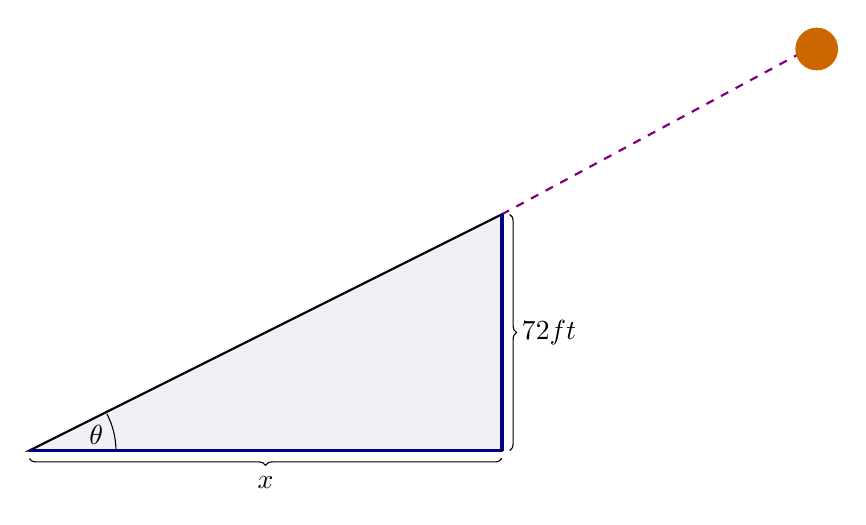
\begin{tikzpicture}
    % \draw[fill1, fill=fill5!50!background] (0,2) triangle (6,5);
             %\draw[fill1, fill=fill1!50!background] (0,0) rectangle (5,5);
      \coordinate (A) at (6,2);
      \coordinate (B) at (6,5);
      \coordinate (C) at (0,2);
     % \coordinate (D) at (2.5,2);
     % \coordinate (E) at (2.5,3.23);
      \coordinate (F) at (0.1,2);
       \coordinate (H) at (0.3,2);
       \coordinate (K) at (0.29,2.1);
      \tkzMarkRightAngle(C,A,B)
     % \tkzMarkRightAngle(C,D,E)
      \tkzDefMidPoint(A,B) \tkzGetPoint{a}
      \tkzDefMidPoint(A,C) \tkzGetPoint{b}
      %\tkzDefMidPoint(D,C) \tkzGetPoint{x}
      \draw[decoration={brace,mirror,raise=.1cm},decorate,thin] (0,2)--(6,2);
      \draw[decoration={brace,mirror,raise=.1cm},decorate,thin] (6,2)--(6,5);
       % \draw[decoration={brace,mirror,raise=.1cm},decorate,thin] (2.5,2)--(2.5,3.23);
        \draw[thick,fill1,fill=fill1!30!background] (A)--(B)--(C)--cycle;
          \draw[thick] (A)--(B)--(C)--cycle;
        \draw[dashed,penColor3, thick] (6,5) -- (9.8,7.05);
         \draw[penColor, ultra thick] (6,2) -- (6,5);
        \draw[penColor, very thick] (0,2) -- (6,2);
      %\draw[thick] (D)--(E)--(C)--cycle;
          % \draw[thick] (D)--(E)--(C)--cycle;
            \draw [very thick,penColor5,fill] (10,7.1) circle [radius=0.25];
             %\draw [thick,penColor] (2.5,3.13) circle [radius=0.1];
      \tkzMarkAngle[size=1cm,thin](H,F,K)
      \node at (3,1.6) {$x$};
       \node at (0.85,2.2) {$\theta$};
     % \node at (2.6,3) {$6$};
      % \node at (3,2.6) {$6ft$};
      \node at (6.6,3.5) {$72ft$};
    \end{tikzpicture}
  \end{image}
  \end{hint}
  
  
  
STEP 2

Complete the following statements.

The known rate is
 \[
\dd t \theta=\answer{ - 0.25} \text{  rad}/hr
\]

The  rate  to be determined is
\[
\dd t \answer{x} \text{    , when    } \theta=\frac{\pi}{6}
\]



STEP 3

Write an equation that relates  all relevant variables.


\[
\tan(\theta)=\answer{72/x} 
\]



STEP 4

Differentiate both sides of the equation above with respect to $t$ (differentiate the left side first)  .


\[
\answer{\sec^{2}{(\theta)}}\cdot \dd t \answer{\theta} =\answer{-72/x^{2}} \cdot \dd t \answer{x} 
\]



STEP 5

Evaluate.
Now, in order to evaluate the equation at the instant when $\theta=\frac{\pi}{6}$, we have to find the value of $x$ at that instant!


\begin{hint}
 \begin{image}
    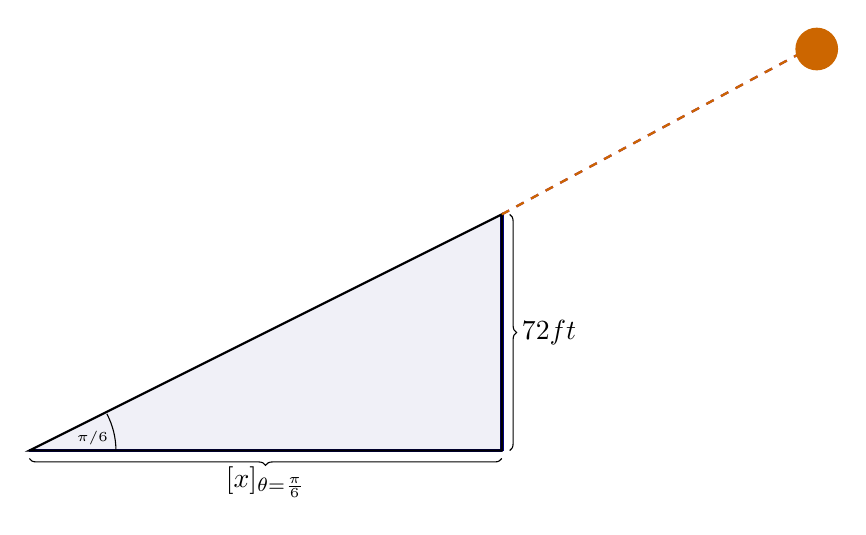
\begin{tikzpicture}
      \coordinate (A) at (6,2);
      \coordinate (B) at (6,5);
      \coordinate (C) at (0,2);
     % \coordinate (D) at (2.5,2);
     % \coordinate (E) at (2.5,3.23);
      \coordinate (F) at (0.1,2);
       \coordinate (H) at (0.3,2);
       \coordinate (K) at (0.29,2.1);
      \tkzMarkRightAngle(C,A,B)
     % \tkzMarkRightAngle(C,D,E)
      \tkzDefMidPoint(A,B) \tkzGetPoint{a}
      \tkzDefMidPoint(A,C) \tkzGetPoint{b}
      %\tkzDefMidPoint(D,C) \tkzGetPoint{x}
      \draw[decoration={brace,mirror,raise=.1cm},decorate,thin] (0,2)--(6,2);
      \draw[decoration={brace,mirror,raise=.1cm},decorate,thin] (6,2)--(6,5);
       % \draw[decoration={brace,mirror,raise=.1cm},decorate,thin] (2.5,2)--(2.5,3.23);
        \draw[thick,fill1,fill=fill1!30!background] (A)--(B)--(C)--cycle;
        \draw[dashed,penColor3, thick] (6,5) -- (9.8,7.05);
         \draw[penColor, ultra thick] (6,2) -- (6,5);
        \draw[penColor, very thick] (0,2) -- (6,2);
      \draw[thick] (A)--(B)--(C)--cycle;
       \draw[dashed,penColor5, thick] (6,5) -- (9.8,7.05);
         \draw [very thick,penColor5,fill] (10,7.1) circle [radius=0.25];
      %\draw[thick] (D)--(E)--(C)--cycle;
          % \draw[thick] (D)--(E)--(C)--cycle;
           % \draw [very thick,penColor5] (10,7.5) circle [radius=0.25];
             %\draw [thick,penColor] (2.5,3.13) circle [radius=0.1];
      \tkzMarkAngle[size=1cm,thin](H,F,K)
      \node at (3,1.6) {$[x]_{\theta=\frac{\pi}{6}}$};
       \node at (0.8,2.16) {\tiny $\pi$/6};
     % \node at (2.6,3) {$6$};
      % \node at (3,2.6) {$6ft$};
      \node at (6.6,3.5) {$72ft$};
    \end{tikzpicture}
  \end{image}
  \end{hint}
  
  
\[
\left[x\right]_{\theta=\frac{\pi}{6}}=\frac{\answer{72}}{\tan{\left(\frac{\pi}{6}\right)}}
\]


\[
\answer{\sec^{2}{\left(\frac{\pi}{6}\right)}}\cdot  \answer{-0.25} =\frac{-\tan^2{\left(\frac{\pi}{6}\right)}}{\answer{72}}\cdot \left[\dd t {x} \right]_{\theta=\frac{\pi}{6}}
\]



STEP 6

Solve for $ \left[\dd t {x} \right]_{\theta=\frac{\pi}{6}}$.

\[
 \left[\dd t {x} \right]_{\theta=\frac{\pi}{6}}=\answer{72}\text{  ft/hr}.
\]
\end{exercise}
\end{document}